\chapter{Performance Evaluation}\label{chap:perfs}

\section{Test application}\label{sec:vpnapp}

As MPDTLS is implemented inside a library, we need an application to use it. We tried to find out an existing application that could be a good candidate for our tests. First, we needed an application which uses DTLS for most of its communications. It was surprisingly hard to find but we still managed to find one : Campagnol\cite{campagnol}. Campagnol is a decentralized VPN solution that uses DTLS to communicate between the peers. Unfortunately, for reasons exposed in Appendix \ref{app:campagnol}, we were unable to integrate correctly our modified library within this application.

So, we took the decision to build a simple VPN application \cite{mpdtls-vpn} by reusing some part of Campagnol code. A VPN application is indeed perfectly suitable for all the experiences we could imagine : potentially any application can use a VPN tunnel without even noticing it. Each packet is encapsulated inside a DTLS packet transmitted securely between the two MPDTLS hosts (see Figure \ref{fig:vpn}).

\begin{figure}[!ht]
\centering
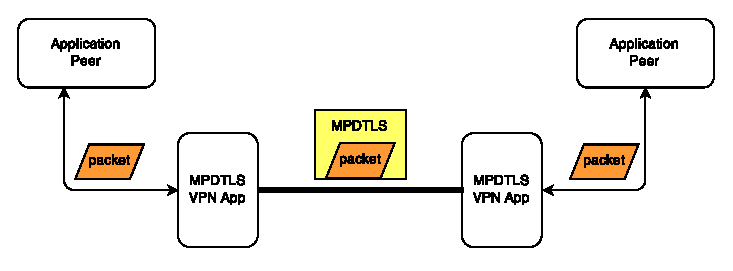
\includegraphics{images/vpn.eps}
\caption{A simple VPN application using MPDTLS}
\label{fig:vpn}
\end{figure}

The behavior of such a MPDTLS VPN App is shown on Figure \ref{fig:vpn-io}. A TUN interface is created with a specified address and netmask. Every packet going to an address falling in this netmask is sent by the kernel to this interface. Then we need to monitor this interface, to read the incoming packets and to sent them through the tunnel. This is the job of the first thread (in red on the Figure). We also need to capture packets coming from the network and to forward them to the TUN interface. This is handled by a second thread represented in green on the Figure. Finally, a last thread (in blue) listens to the standard input for potential commands. This is the channel that we use to communicate with the application to add or remove new interfaces for instance. We can ask for debug information or even change the scheduler policy on the fly.

\begin{figure}[!ht]
\centering
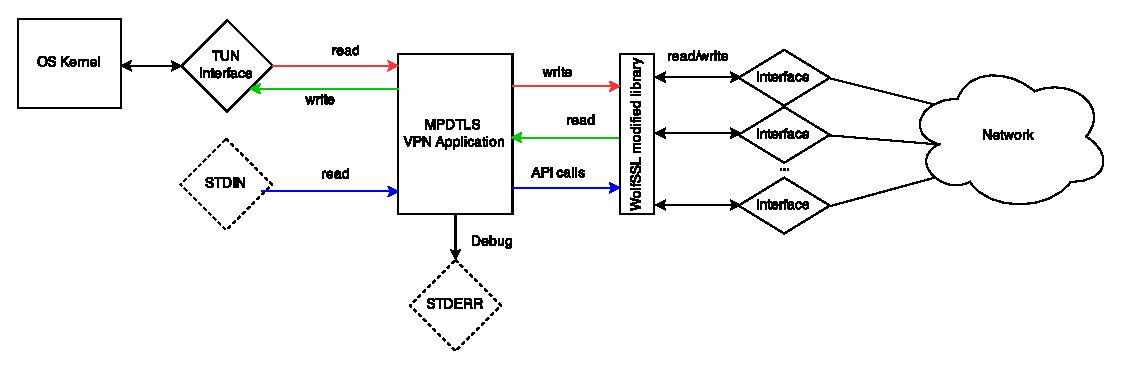
\includegraphics[width=\textwidth]{images/tunneling-IO.eps}
\caption[I/O interactions for one host of our application]{I/O interactions for one host of our application. Each thread is represented with one color.} 
\label{fig:vpn-io}
\end{figure}

One of the most useful information we can ask for are the statistics for a particular flow. Looking at this output, we can identify most of the time an issue without analyzing at the packet trace. An example of such an output is shown on Listing \ref{lst:stats}. We can easily see the part of the traffic that the subflow is actually supporting, the estimated delays and other information. The separator "|" used in the \texttt{packets sent} list differentiates the ones that are in the waiting status and the others (see Section \ref{sec:impl-stats} for more details about this waiting status).

\begin{lstlisting}[language=bash,caption=An output of the statistics for a particular flow,label=lst:stats]
---- Stats Flow N 0 ---- 
IP src : 11.0.0.1 
IP dst : 11.2.0.1 
Support 41 % of the connection
----- Receiver Stats ----- 
Packets received : 44 
Min_Seq received : 76 
Max_Seq received : 172 
Backward delay : 10 ms
----- Receiver Cache ----- 
Packets received : 0 
Min_Seq received : 2147483647 
Max_Seq received : 0 
----- Sender Stats ----- 
Packets sent : [ 8487 8489 8492 ... 8633 8634 8636 | 8640 8642 ... 8706 8707] 
Forward delay : 10 ms
Loss Rate : 0.000000 
---------------------------

\end{lstlisting}

\section{Different scheduler policies}\label{sec:perf-sched}

We present here three examples of scheduler strategies that we have implemented and how the fractional distribution is computed in each case. As conclusion, each of them has pros and cons. The good choice is strongly related with what the underlying application expects to do. In some cases, an application could want to build its own scheduler and this matches with our design since we provide a dedicated customisable callback.


\subsection{\texttt{Round Robin}}

The round robin is the simplest strategy consisting in sending the same amount of packets over each available link. This does not use any of the information gathered from the feedback. However it may be a good choice if we know in advance that the different links share common properties (e.g. in a datacenter).

The fractional distribution is really easy to compute as every link will get the same fraction of the traffic (in terms of number of packets).

\begin{equation*}
f_i = \frac{1}{n}
\end{equation*}

where $f_i$ is the portion of traffic given to flow $i$ and $n$ is the total number of subflows.

\subsection{\texttt{Optimize Latency}}

For this strategy, we want to give more weight to the links where the forward delay is lower. We have to keep in mind that every delay $d_i$ contains the clock desynchronization term $\Delta T$ (see Section \ref{sec:forward-delay}). In order to get rid of this term, we must consider the difference with another delay. We choose to take the difference with the maximum delay as by definition the greater the difference, the smaller the delay. This maximum will evolve and is defined as the maximum delay reported on every flow at the time we compute this fractional distribution. Equation \ref{eq:latency} gives the complete expression.  

\begin{equation}
f_i = \frac{max_d - d_i + \alpha}{\sum_j (max_d - d_j) + n*\alpha }\quad \text{where } \quad max_d = max_i(d_i) 
\label{eq:latency}
\end{equation}

Without the $\alpha$ term, the flow with the maximum delay will never be used. Indeed if you have two subflows with forward delays of 10ms and 20ms and $\alpha=0$, then $100\%$ of the traffic will be supported by the first subflow. Although this could appear as an optimal choice, it is always preferable to send a small part of the traffic on each link just to monitor the characteristics and to keep receiving feedback and heartbeat messages. After some tests, we think the value of $\alpha$ must be defined between 5\% and 10\% of $max_d$\footnote{Of course, $max_d$ must not be null. If it is the case, then a constant value must be chosen like 1ms and the equation will actually give the same result as a round robin.} to give the best results. 

\subsection{\texttt{Optimize Loss}}

Another strategy that we could consider is to favor the less congested links. In this case, we give more priority to a link with the smallest loss rate. The principle is almost the same as for the latency, we consider the difference with the biggest loss rate observed. The idea is to quantify the relative differences between the subflows.

We may be tempted to use directly the loss rate reported in the statistics. However if the link experiences severe losses, we may not be aware of it because all the feedback packets have been dropped. Therefore we compute what we call the "real" loss rate which also takes in consideration the number of packets sent and not yet acknowledged. Equation \ref{eq:lr} gives the formula used and $feedback_{thr}$ is the number of packets after which we send a feedback. We consider two times this amount to give a penalty to the link because after one feedback, packets are in waiting status and need another feedback before being completely forgotten. The penalty $pen$ is computed as two times the probability of loosing one feedback. The factor $2$ here will probably need some tuning but the idea is to boost the penalty as the risk is rather small to loose only the feedback packet but no application data. 

\begin{align}
LR_i &= stats_{LR} + \left \lfloor{\frac{pckts_{sent}}{2 * feedback_{thr}}} \right \rfloor  * pen & \text{where } \quad pen = \frac{1}{feedback_{thr}} * 2 \label{eq:lr} \\
f_i &= \frac{max_{LR} - LR_i + \beta}{\sum_j (max_{LR} - LR_j) + n*\beta } & \text{where } \quad max_{LR} = max_i(LR_i) 
\label{eq:losses}
\end{align}

Equation \ref{eq:losses} is really similar to Equation \ref{eq:latency} and we also need a constant term $\beta$ for the same reasons. After some tests, we arrive at the conclusion that a suitable value for $\beta$ is around $1\%$  of the loss rate in most situations.

\section{Multipath simulations}

We have designed an environment to evaluate our system under different conditions. All the following measures take place inside a Mininet laboratory \cite{mininet} to easily set up the topology we want and to create multiple interfaces. Also, we used a kind of framework for Mininet called Minitopo\cite{minitopo} to easily configure the topology and create automated tests just with configuration files instead of scripts. To generate network traffic, we used the D-ITG (Distributed Internet Traffic Generator)\cite{ditg} tool. More details about how to reproduce these graphs and the following are given in Appendix \ref{app:graph}.

\subsection{Topology}\label{sec:perftopo}

The topology used for the following evaluations is the one presented on Figure \ref{fig:topo-phys}. We have four interfaces on the client side that are linked to a network router and one link between the router and the server. Note that the latter is not constrained, we will only change the characteristics of the first 3 paths shown on the Figure. The path 4 is reserved for the signaling of D-ITG to avoid any interference with our measures.


\begin{figure}[!ht]
\centering
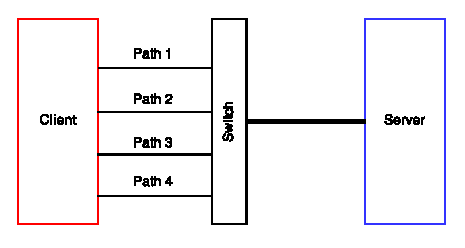
\includegraphics[width=0.7\textwidth]{images/perf-topo-phys.eps}
\caption{Physical topology inside mininet}
\label{fig:topo-phys}
\end{figure}

The corresponding logical topology is depicted on Figure \ref{fig:topo-log}. We are using 3 flows concurrently between the client and the server. The D-ITG application is sending traffic to one unique TUN interface and the traffic goes through our tunnel to reach the D-ITG receiver.

\begin{figure}[!ht]
\centering
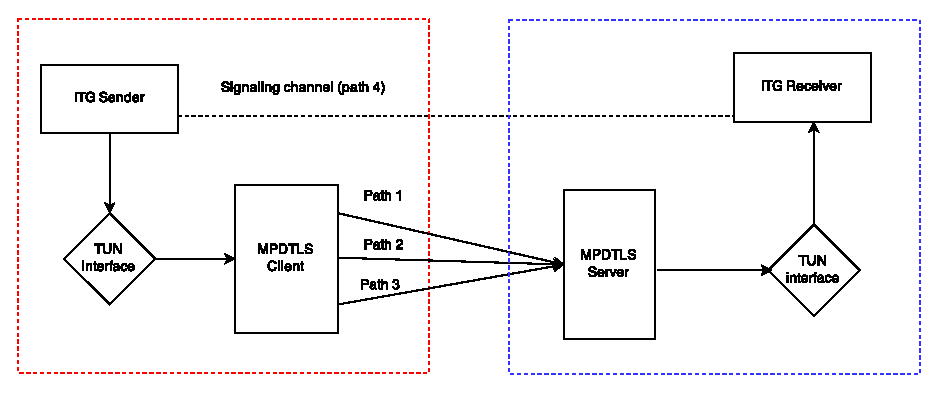
\includegraphics[width=\textwidth]{images/perf-topo-logic.eps}
\caption{Logical topology used for measurements}
\label{fig:topo-log}
\end{figure}

\subsection{Traffic balancing}

The first thing to evaluate is if we really take advantage of multiple interfaces and how we balance the traffic between them. We performed experiments to determine in which conditions each scheduler works well and how they compute the distribution of traffic in various environments.

\subsubsection{With dynamic bandwidth}

In this experiment, we have tested the two schedulers that are taking the context into consideration : \texttt{Optimize Latency} and \texttt{Optimize Loss}. The configuration used is the following (the path indexes refer to Figure \ref{fig:topo-log}) :


\begin{center}
\begin{tabular}{|c|c|c|c|}
\hline
Path n\degree & bandwidth & loss rate & delay  \\ \hline
1 &  1 Mbps & 0 & 10ms \\ \hline
2 & variable & 0 & 20ms \\ \hline
3 & not used & - & - \\ \hline
\end{tabular}
\end{center}

We ran the experiment with multiple values of bandwidth of path 2 to see how its usage rate is impacted. We have generated constant traffic with D-ITG \cite{ditg} using both UDP and TCP. All these results are reported in Figure \ref{fig:dynbw}. The measurements have been obtained with sessions of 60 seconds and every experiment has been repeated 11 times to evaluate the mean. The 95\% confidence interval of the mean is presented in white and has been computed with a Student T distribution.


\begin{figure}[!ht]
\centering
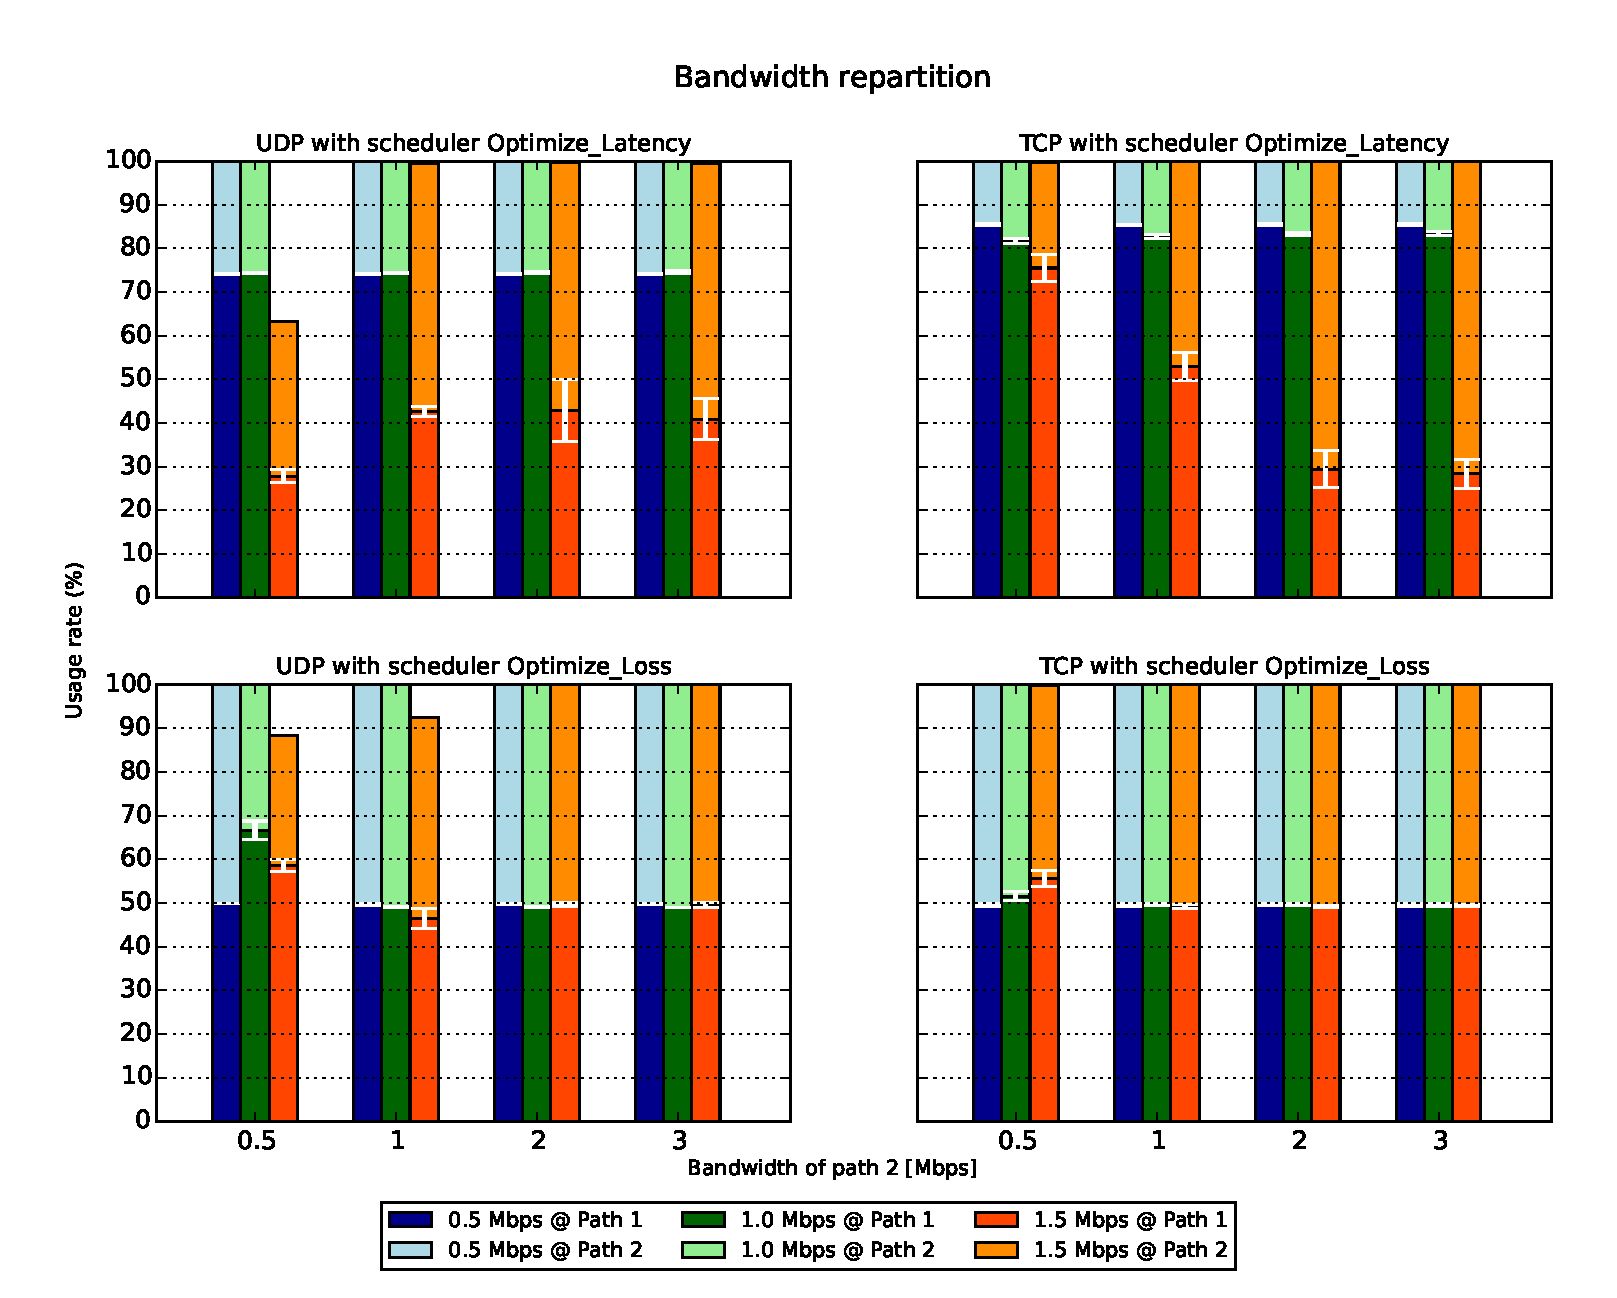
\includegraphics[width=\textwidth]{images/xp/graph1.eps}
\caption{Usage repartition with bandwidth variation}
\label{fig:dynbw}
\end{figure}


For every bandwidth value of path 2, we have 3 bars that represent the total traffic we are trying to send through the tunnel. Each bar is separated in two parts that show the amount of traffic passing through each path in bytes/sec. The losses are easily identifiable because they occur every time the total usage does not reach the total bandwidth. Of course at the beginning we have congestion because if path 2 can support only $0.5Mbps$ then $bw(p1) + bw(p2) = 1.5Mbps$ and in the last case we are trying to send traffic at 1.5Mbps. So, it is supposed to use 100\% of the tunnel capacity which is impossible in practice. Moreover, this computation does not even take into account the overhead introduced by the encapsulation inside DTLS. Indeed, we are sending packets of size 825 bytes into the TUN interface and the resulting size of the DTLS \texttt{ApplicationData} packet is 905 bytes; so an overhead of 80 bytes (almost 10\% in this case).

First, it is interesting to confirm that the \texttt{Optimize loss} scheduler performs better if we are dealing with congested links and especially with UDP. Note that TCP doesn't experience losses in the same way as UDP because it will reduce its transmission rate internally with the congestion window mechanism. So even if we impose a given volume of traffic, the real bandwidth will be lower with TCP in case of congestion.

Secondly, we observe an unexpected phenomenon if we look at the graph "UDP with scheduler Optimize Latency" : when we increase the total bandwidth to 1.5Mbps (orange), it does not optimize latency at all. Indeed, it gives only a small part of the traffic to the faster link. We have tracked down the problem and it is apparently coming from a bad perception of the forward delay. At the beginning, it uses extensively path 1 as expected but rapidly reaches congestion as the capacity of path 1 is 1Mbps. The heartbeat messages that are used to evaluate the forward delay are themselves postponed by a few milliseconds due to this congestion and it is sufficient for the scheduler to estimate the delay is better on path 2. Even if the forward delay is later correctly estimated, we go back in the same cycle.  It is not the case with TCP at least at the beginning because TCP reduces the bandwidth to fit into the tunnel and therefore there is no congestion observed.

\subsubsection{With dynamic loss rate}\label{sec:perfs-loss}

This time, we want to see how the schedulers react with various loss rate at one of the paths. The configuration is the following :

\begin{table}[!ht]
\centering
\begin{tabular}{|c|c|c|c|}
\hline
Path n\degree & bandwidth & loss rate & delay  \\ \hline
1 &  1 Mbps & 0 & 10ms \\ \hline
2 & 3 Mbps & variable & 10ms \\ \hline
3 & not used & - & - \\ \hline
\end{tabular}
\end{table}

Again we are using 2 paths only and they have the same latency but different bandwidths. We run different experiments with 4 values of loss rate for path 2, going from 0\% to 3\%. The results we have obtained are presented on Figure \ref{fig:dynloss}.


\begin{figure}[!ht]
\centering
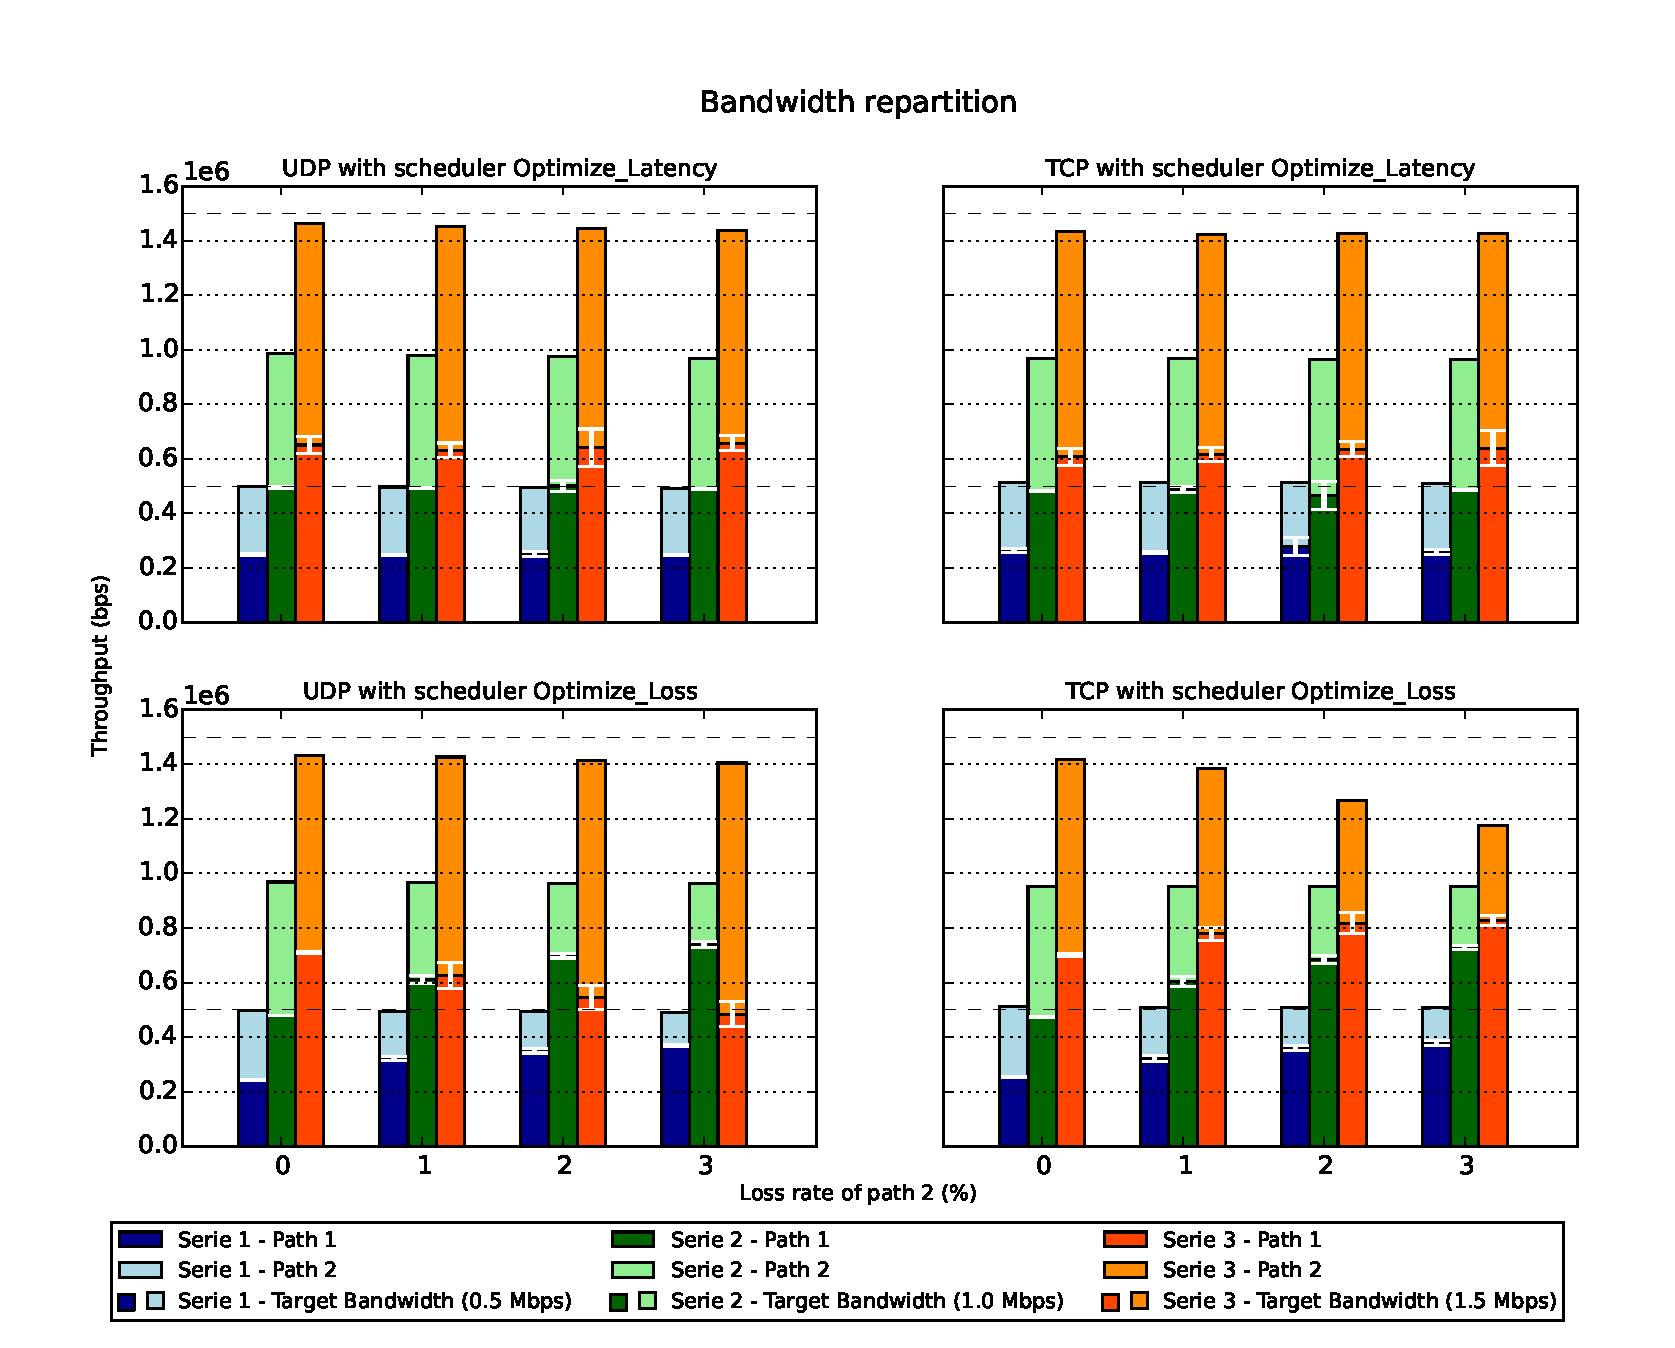
\includegraphics[width=\textwidth]{images/xp/graph2.eps}
\caption{Usage repartition with loss rate variation}
\label{fig:dynloss}
\end{figure}

A first element to point out is the fact the \texttt{Optimize Latency} scheduler is not really impacted by the loss rate as we could expect. The proportion is always around 50\% for both TCP and UDP as the two links have the same delay. The little exception to this rule is noticed for the third bar (traffic at 1.5Mbps) probably because we reach the congestion limit on path 1. Therefore, the heartbeat messages are either delayed or dropped and the forward delay is overestimated.

On the other side, the \texttt{Optimize loss} scheduler will progressively give more weight to the first path as it is loss free. We state that UDP and TCP give different results concerning the last bar which corresponds to the 1.5 Mbps transfer speed. Again, this can be explained by the congestion on path 1. UDP keeps sending packets even if they are dropped, therefore the scheduler will detect important losses on path 1. The loss rate caused by congestion will overcome the one of path 2 and the scheduler will thus choose the best option among the two. However, for TCP, the congestion control mechanism will reduce the sending rate to avoid congestion of path 1. In such conditions, path 1 remains the best option and thus receives more weight from the scheduler.


\subsection{Resiliency to interface removal}

The objective of using multipath is not only to balance the traffic on the existing paths but also to modify dynamically the distribution of the traffic if one interface becomes unavailable. For this experiment, we use the topology of Figure \ref{fig:topo-log} with the following configuration : 

\begin{table}[!ht]
\centering
\begin{tabular}{|c|c|c|c|}
\hline
Path n\degree & bandwidth & loss rate & delay  \\ \hline
1 & 5 Mbps & 0 & 10ms \\ \hline
2 & 5 Mbps & 0 & 20ms \\ \hline
3 & 5 Mbps & 0 & 40ms \\ \hline
\end{tabular}
\end{table}

We generate constant UDP traffic at 3 Mbps and observe the behavior of the implementation if path 1 is suddenly broken at $t=19s$. The bandwidth repartition is shown on Figure \ref{fig:xp-lossint-bw} and the scheduler used is \texttt{optimize loss}.


\begin{figure}[!ht]
\centering
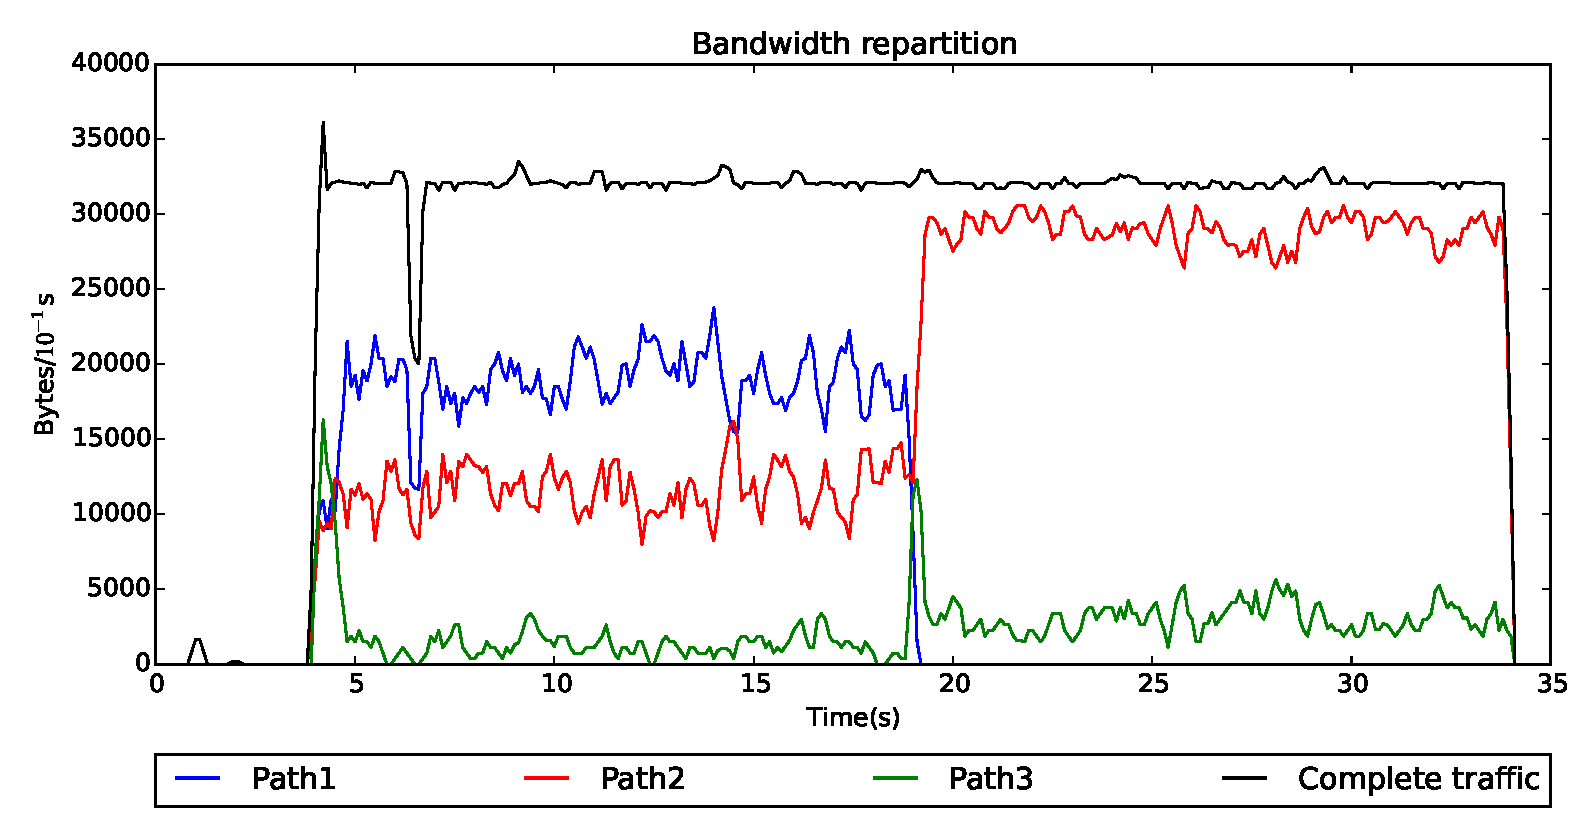
\includegraphics[width=\textwidth]{images/xp/intlost_bw.eps}
\caption{Reaction to interface removal}
\label{fig:xp-lossint-bw}
\end{figure}

Note that the path 1 was used for the handshake and we prove here that even if we remove our "primary" interface, the connection continues. In the very first moments (at 4s), we note that the distribution is more or less equal among the subflows. This setup time is needed to obtain some information about the forward delay. Heartbeat messages and feedback packets have to be exchanged between the two hosts. After 5 seconds, we see that the distribution is shaped with what we can expect from Equation \ref{eq:latency}: path 1 has almost $2/3$ of the traffic because it has the best delay, path 2 is still used because the difference of delays with path 1 is acceptable and then some traffic is given to path 3 to monitor the link. Of course, a more aggressive scheduler will probably let path 1 support 100\% of the traffic but the objective here was to use all paths to perform probing.

When path 1 fails, the distribution is recomputed and most of the traffic is re-routed to path 2. Of course we are far from the congestion because each link has a bandwidth of 5 Mbps but the objective here was to see how the distribution is moving without other constraints. In this context, the scheduler is doing well by optimizing the overall latency as we can see in Figure \ref{fig:xp-lossint-delay}. After the loss of the fastest path, the overall delay is increased and is little above the  20ms threshold which is the delay of the new fastest link. We also can observe two peaks: the first one is due to the setup time and the second one is a temporary increase of path 3 usage to compensate the failure of path 1.



\begin{figure}[!ht]
\centering
\begin{minipage}{0.4\linewidth}
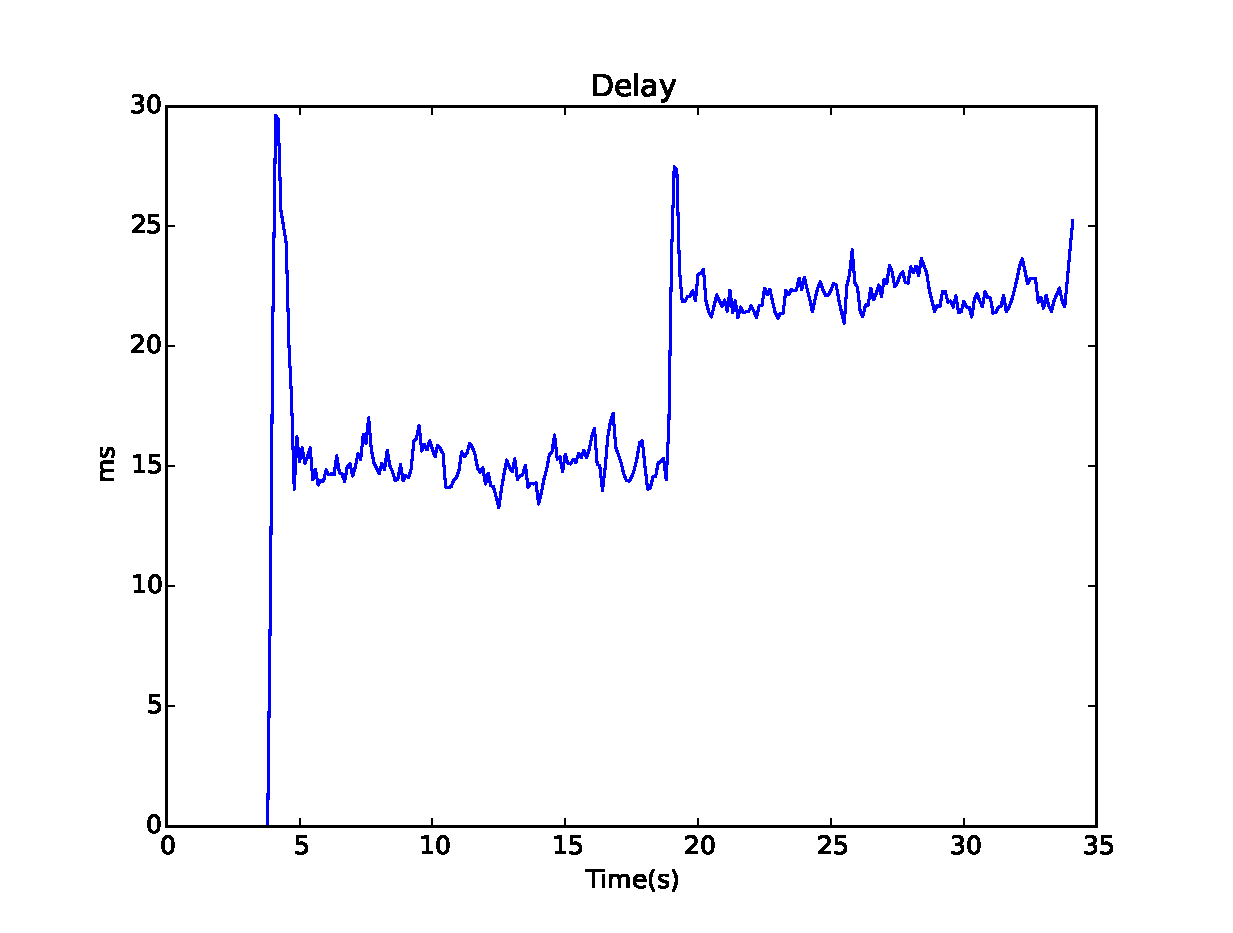
\includegraphics[width=\textwidth]{images/xp/intlost_delay.eps}
\caption{Overall delay}
\label{fig:xp-lossint-delay}
\end{minipage}
\begin{minipage}{0.59\linewidth}
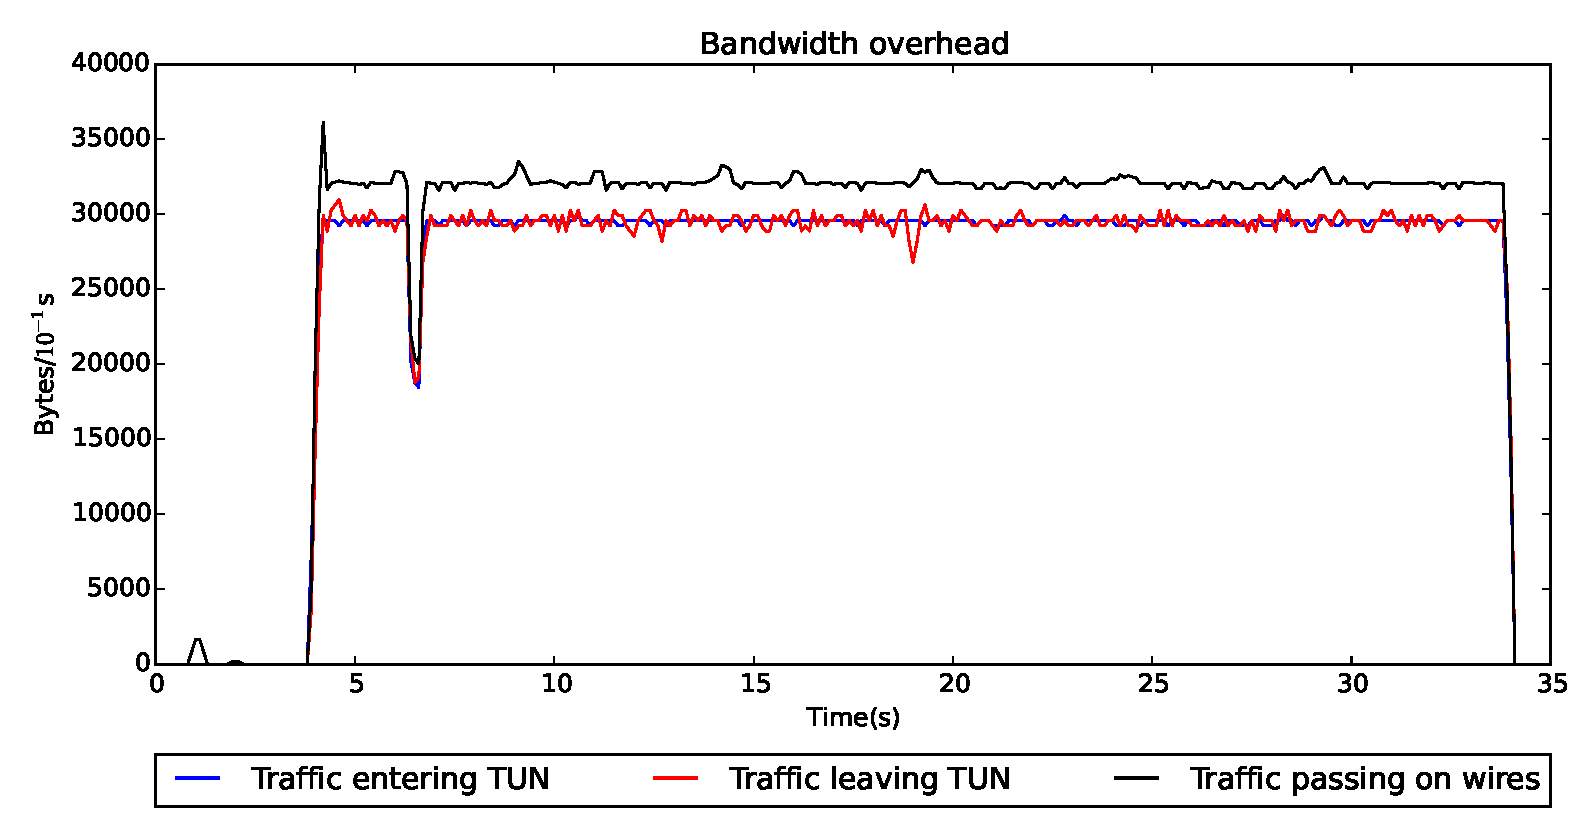
\includegraphics[width=\textwidth]{images/xp/intlost_tun.eps}
\caption{Application perception of traffic}
\label{fig:xp-lossint-tun}
\end{minipage}
\end{figure}

From the application's point of view, the impact of such failures is shown in Figure \ref{fig:xp-lossint-tun}. We see in blue the traffic entering the tunnel which is constant here because we have parametrized D-ITG to do so, in red we see the traffic leaving the tunnel and in black we have the traffic generated by the tunnel. The difference between the blue and the black curves is the overhead caused by the encapsulation of D-ITG packets inside DTLS ones. Around the $19^{th}$ second, we notice a really small drop on the red curve, exactly when the interface was lost. This is the only thing the application will perceive from the loss of one interface. This is a huge improvement in comparison with a normal DTLS connection, which would have ended the communication in case of such interface loss.

\begin{figure}[!ht]
\centering
\end{figure}

\subsection{Smooth addition of a new interface}

In this section, we explore the reverse scenario: when one interface becomes available. At the beginning only path 1 and path 2 are available and at time $t=30s$ we add path 3. The configuration used is the following :

\begin{table}[!ht]
\centering
\begin{tabular}{|c|c|c|c|}
\hline
Path n\degree & bandwidth & loss rate & delay  \\ \hline
1 & 5 Mbps & 0 & 30ms \\ \hline
2 & 5 Mbps & 0 & 40ms \\ \hline
3 & 5 Mbps & 0 & 10ms \\ \hline
\end{tabular}
\end{table}

As we can see path 3 has the lowest delay and we expect that it will take the lead over the two other ones. This is verified with our experiment as we can see on Figure \ref{fig:xp-addint-bw}. A significant portion of the traffic is redirected through the new flow. At the beginning path 1 was the fastest link so it was given the largest part. But after the addition of the new interface, a re-computation is made according to equation \ref{eq:latency} and path 1 is less used.


\begin{figure}[!ht]
\centering
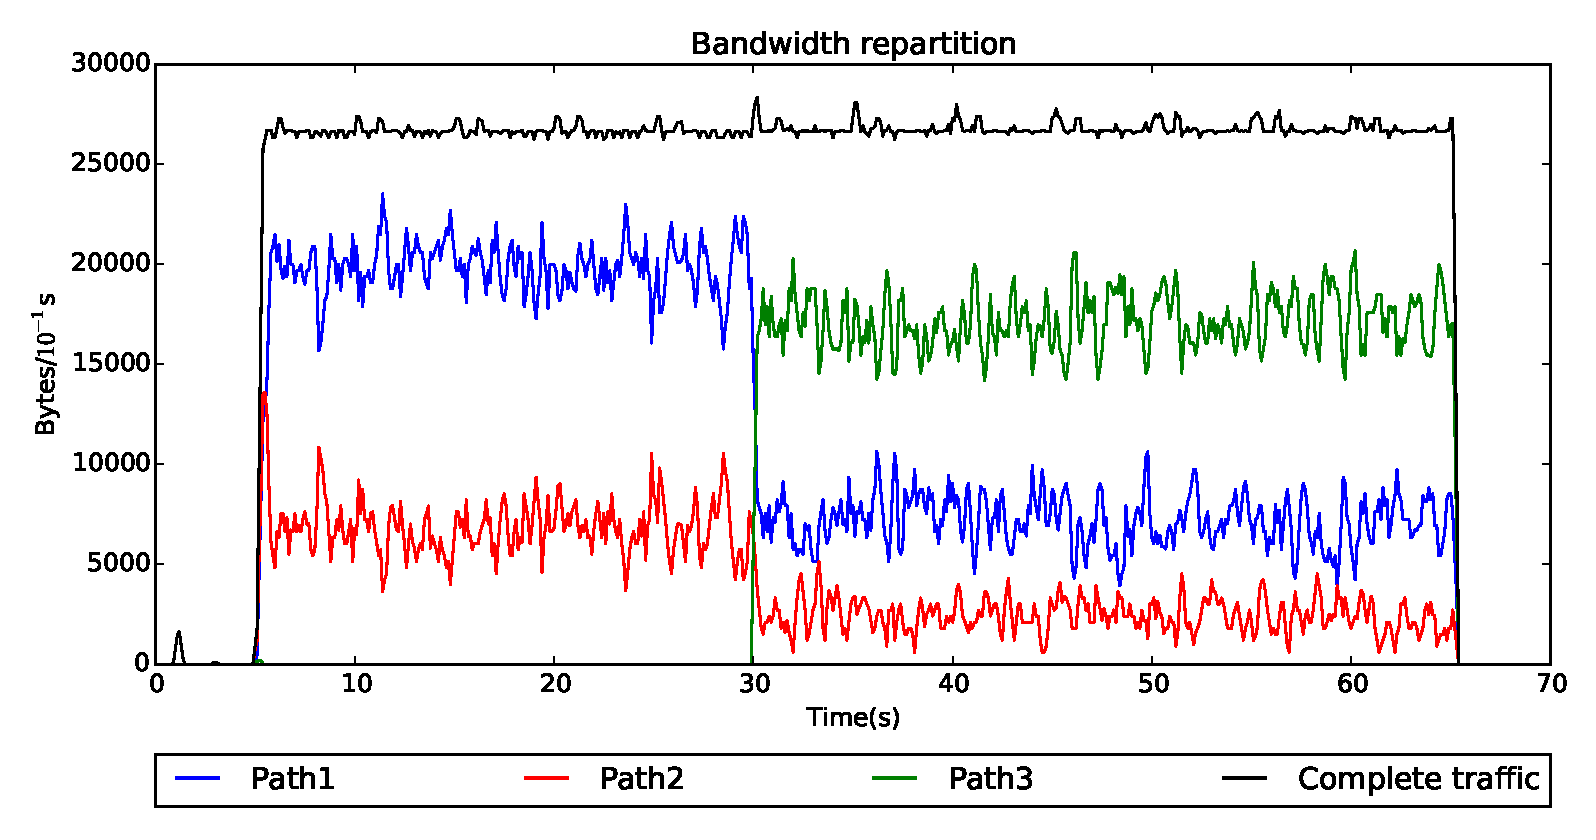
\includegraphics[width=\textwidth]{images/xp/addint_bw.eps}
\caption{Reaction to new interface addition}
\label{fig:xp-addint-bw}
\end{figure}

The overall delay is kept reasonably small according to Figure \ref{fig:xp-addint-delay} but we could probably optimize even more. That would imply putting more weight to path 1 and thus offloading the two other flows. However this is a choice we made to keep using all the paths while still trying to give more traffic to the faster link. It allows faster recovery if the best interface is lost.

\begin{figure}[!ht]
\centering
\begin{minipage}{0.4\linewidth}
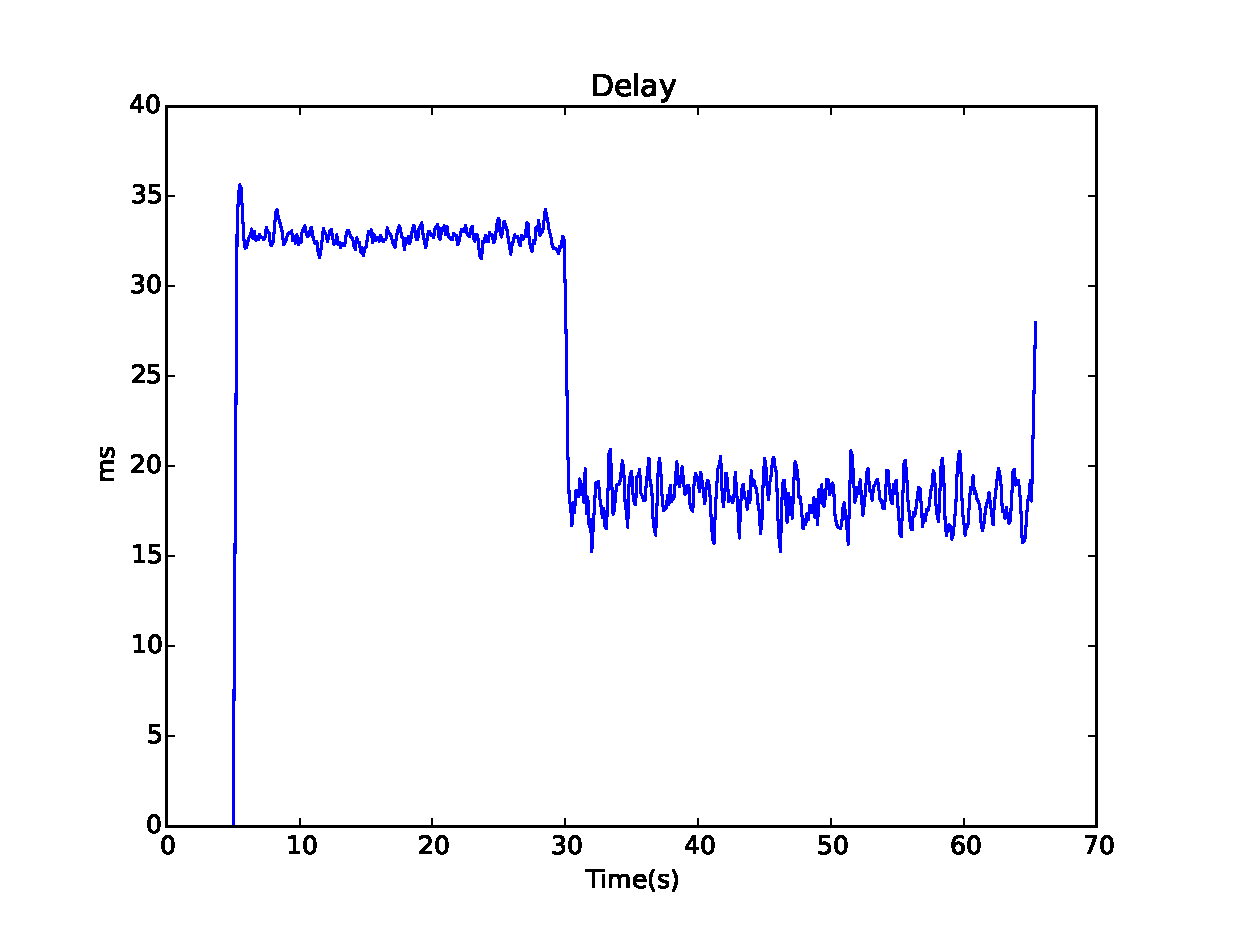
\includegraphics[width=\textwidth]{images/xp/addint_delay.eps}
\caption{Overall delay}
\label{fig:xp-addint-delay}
\end{minipage}
\begin{minipage}{0.59\linewidth}
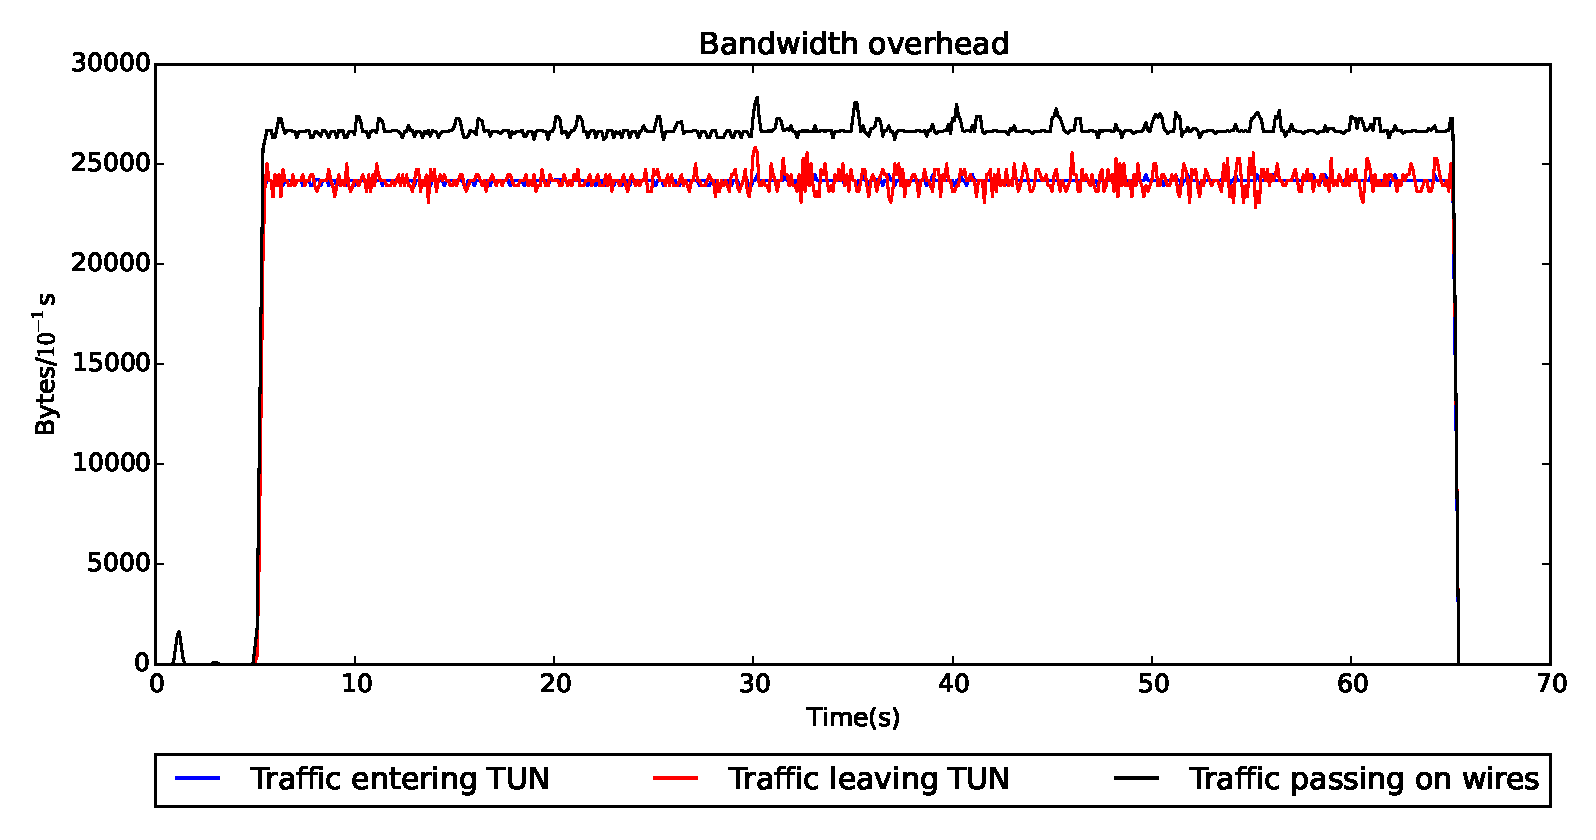
\includegraphics[width=\textwidth]{images/xp/addint_tun.eps}
\caption{Application perception of traffic}
\label{fig:xp-addint-tun}
\end{minipage}
\end{figure}

If we look at the traffic perceived by the application on Figure \ref{fig:xp-addint-tun}, we notice no real perturbation around $30s$. Although the traffic is a bit noisy after this time, this is explained by the fact we have 3 different paths with 3 different delays and therefore packets cannot arrive at a constant rate.

\section{Conclusion}

In this chapter, we have presented a simple VPN application that we have designed to evaluate our MPDTLS implementation. To dispatch efficiently the packets between the available flows, 3 schedulers have been created : \texttt{Round Robin}, \texttt{Optimize Loss} and \texttt{Optimize Latency}. We have concentrated our evaluation on the last two since the \texttt{Round Robin} doesn't consider any contextual information. 

After various experiments, we have shown that the \texttt{Optimize Latency} scheduler behaves better when there is no congestion. Otherwise, it tries to push a large amount of traffic on the faster link and quickly triggers congestion. However, we have discovered that the counter-reaction will avoid too many losses. As the additional delay caused by the congestion will increase the perceived latency, the scheduler will therefore redirect the traffic through other paths.

On the other side, the \texttt{Optimize Loss} scheduler behaves better when there is congestion or simply if one link looses more packets than another one. This would typically be the case for a Wi-Fi interface in an environment with interference. In such case, the most reliable link is preferred as long as it is not congested.

In addition, we have shown that an application using our MPDTLS tunnel will not be much troubled if one interface is lost in the middle of the communication. This is also the case if we add a new interface on the fly.






 